%update: Jan 15 fixed grammar according to prof notes.
%update: Jan 13 added a figure of solar cell. 
%update: Jan 09-11 prof check
%update: Dec 20 finished writing. 

%\begin{savequote}[75mm] 
%In three words I can sum up everything I've learned about life: it goes on.
%\qauthor{Robert Frost} 
%\end{savequote}

\chapter{Conclusions and Future Perspectives}

\newthought{In summary}, probing technique is applied to nanomaterials using \emph{in situ} TEM with many factors considered, such as chemical transitions, physical (electrical and mechanical) contacts and light illuminations. 
I reviewed and introduced related research in {\it in situ} probing TEM of nanomaterials for flexible optoelectronics and ion batteries applications in Chapter 1. 
Then the engineering details are discussed and presented in Chapter 2. 
Some behaviours or performances are revealed and discussed in Chapters 3-6, I finally summarize them herein and express my views of the future prospects based on my detailed understanding due to my PhD research experience. 

\section{Conclusions}
%chapter 3 revised
In Chapter 3, a direct and powerful {\it in situ} probing \textit{nanoarchitectonics} technique to construct individual axial nanowire junctions has been for the first time realized. 
{\it In situ} HRTEM and in-tandem crystallography characterizations and optoelectronic behavior studies uncover the optical sensing properties of the single-crystalline axial CdS/p-Si nanowire junctions. 
The junctions exhibit decent selectivity toward the light wavelength shorter than those of the yellow range. 
It is very interesting that the junctions hold specific photocurrent saturation effect. 
The saturation of photocurrent at a relatively large bias could be utilized for the low power consumption light intensity sensing and integrated tunable voltage-driven devices, thanks to the corresponding current limitations and excellent tolerance toward some unreliable/unstable biases. 
Obviously, the present {\it nanoarchitectonics} approach employing {\it in situ} structural design and measurements gives hope for the timely establishing detailed operational principles of bottom-up nano-devices. \\

%chapter 4 revised
In Chapter 4, the designed phase-transformation route was found to be successful for fabrication of an N doped graphene-phosphorous anode material with layered sandwich-like morphologies where very thin amorphous red P layers are placed within flexible and conductive N-doped graphene frameworks.\\
Advantages of the as-designed anode material have been studied by various characterization techniques, device tests, {\it in situ} microscopy and theoretical calculations. 
These advantages are: \\
(1) Thin P layer on the doped graphene (instead of crystalline P) anode shows ultrastable efficiency of 0.002\% decay per cycle and good rate capability of 809 mAh/g at 1500 mA/g; \\
(2) P-C stable bonds may exist to tighly bind GN and P layers; \\
(3) {\it In situ} HRTEM experiments verified and revealed the reasons behind the ultrastable performance.\\

%chapter 5 revised
Chapter 5 discusses on the opto-mechano-electrical tripling phenomenon under {\it in situ} observation and probing measurements of photocurrents in zinc oxide nanowires in real time, and under high spatial resolution. 
By comparing photocurrent spectra of individual free-standing zinc oxide nanowires under strains, splitting of photocurrent spectra is established. 
The shifts of photocurrent peaks are in obvious correlation with the bending strains. 
The red/blue shifts are proved to be directly related to the splitting of energy levels in the valence band at $\Gamma$ point. 
DFTB calculations show a perfect match with the {\it in situ} probing experimental results. 
The splitting of photocurrent spectroscopy provides an important information for future flexible optoelectronics and piezo-phototronics. 
For example, this can be considered for strain tuned wavelength-division multiplexing modules or MOEMS devices, and for flexible optoelectronic components where photocurrent splitting value should be evaded as a key variable. \\

%chapter 6 revised
In Chapter 6, I have successfully performed photocurrent measurements for elastically deformed CdS nanowires inside the HRTEM. Using {\it in situ}  probing technique and light illumination, I have characterized the electronic (dark current) and optoelectronic features of individual nanowires under mechanical deformation. 
To make the data reliable for future bottom-up applications, a large variety of nanowires was measured, which made possible an accurate statistical analysis of their properties. 
All nanostructures reveal similar ON/OFF ratios in original, bent and recovered states, with a value mainly locating from 7 to 20. 
Photocurrent spectroscopy of several nanowires possess red shifts of cut-off wavelength of several nanometers. 
These tiny shifts are mainly caused by deformation induced strains, which result in changes in the electronic band structure. 
By taking SAED patterns, the strain-induced structural deformation was confirmed after bending. 
The experiments reveal a variety of bending-induced stability for individual nanowires. However, from a statistical point of view, the nanowires display common features in their response to deformation, making them valuable for future flexible optoelectronic applications. \\

\section{Future perspectives}
%%%%%%%%%%%%%%%%%%%%%I guess this subsection is unnecessary%%%%%%%%%%%%%%%%%%%%%%%%%%%%%%%%%%
%\subsection{Look back to history to see where we are}
%Anthropologist believe that an evolution of mankind would be linked to the use of tools. \cite{lilley1948men} The ancients made tools to handle things at a meter scale, such as knife, wrench, scythe, sickle. Human civilization history is very much related to to development of tools. By updating tools, humankind was able to handle meter scale objects, and gradually went down to a few scales different from our size. The advancement of tools development is directly determined by the development of science and technology. 

%From millions of years ago, humankind started to updating tools. During prehistroy (before 3,000 BC) and ancient age (3,000 BC to 476 AC), more and more well the stones were machined, bronze and iron made tools came out to serve human beings for daily use - at a scale from centimeter to hundred of meters. In the paleolithic age, people were mainly making simple tools; while in the neolithic age, people became experienced with applying tools to building constructions. The capability of human beings are still restricted withing 3 scales from ourselves. It is called {\it meter-scale age}. 

%In the medieval age (476 AC to 1492 AC), the development of classical optics, including the production of well-made lenses, laid the groundwork for microscopy - the tool to reach microscale and astronomical scales. In modern age (1492 AC to 1789 AC), many revolutionary researches in optics and microscopy were associated and contributed to the fast development of physics, chemistry, biology and material science. It is called {\it micro-scale age}. 

%During the last century, development of particle physics, theory of relativity and quantum mechanics made it possible to see nanoscale world by electron microscopy and atomic force microscopy. It is called {\it nano-scale age}.

%The important mark between each "scale age" is the invention of an optical microscope and an electron microscope, because the preliminary important thing to do with the scale is to see objects in that scale. The main activities at the early stage of each "scale age" were development of the microscopy itself, as well as observing and getting knowledge of the new world objects. The main activities at the second stage of each "scale age" is the production of building blocks and their applications in those scales. Only when people become very familiar with almost everything in that scale with daily used applications, then science advances might move to the next scale via rising theories and making experiments. 

%After developing precised mechanics, humans became able to make fine mechanics to operate with the small objects. The gear was able to transfer a larger movement into fine movements. The ratio could be improved by the development of advanced gearing. However, it is not until recent years that people became capable to reach nanometer precision with mechanics once a piezoelectric motor has been invented. \cite{} 

%Clearly we are now in the cross road between the first stage and second stage of the {\it nanoscale age}. 

%%%%%%%%%%%%%%%%%%%abandoned paragraph, although I like it...%%%%%%%%%%%%%%%%%%%%%

\subsection{Nanoscale building blocks in future}
Although many researchers always claim that their nanomaterial samples are perfect and uniform, the quality is not that perfect to clarify on identical physical or chemical properties.\\

In Chapter 3, we noticed that the reproducibility (Table 3.1) is very high for heterojunctions with respect to the discovered saturation effect. 
But the current values vary a lot based on different sizes of building blocks. 
In Chapter 6, it is noticed that even the ratios of photo-to-dark current ratios in different states are more or less stable, the photo-to-current ratios of each nanowire are very different from each other. 
The scattered distribution of the ratios is caused by non-uniform structural features and chemical compositions. 
To use the nanowires in bundles is practical in some applications, while it is not practical to apply them in a single nanowire device for the mass production. \\

It is expected that nanoscale building blocks can be really uniform at the nanoscale. Such nanoscale building blocks become the bricks for the follow-up architecture. When the synthesis of various nanoscale building blocks can be well controlled to reach identical morphology, surface, physical, and chemical properties, the manufacturing process will become reliable and reproducible. \\

Another problem is that the current understanding of many nanomaterials is not yet comprehensive. But if the materials are synthesized with the identical morphology and crystallography, their properties are easier to be understood. 

\subsection{Nanomanipulations in microscopy in future}
We are now in 2017, the age of nanotechnology, gene engineering, information technology, artificial intelligence and many more striking discoveries. According to the history of tools, human beings are now quite new to the nanometer scale. The tools we are using for the nano-world are electron microscopy, atomic force microscopy, lithography, piezoelectric probing and other technologies. It is true that various nanostructures are indeed successfully synthesized these days, they may be designed on electronic chips for mass production, and their observations may be performed at the atomic resolution. However, lithography technology does not work for many other applications, microscopy has sampling limitations, mechanical technology is not mature yet to handle nanoscale building blocks easily. 

\begin{figure}  
\centering
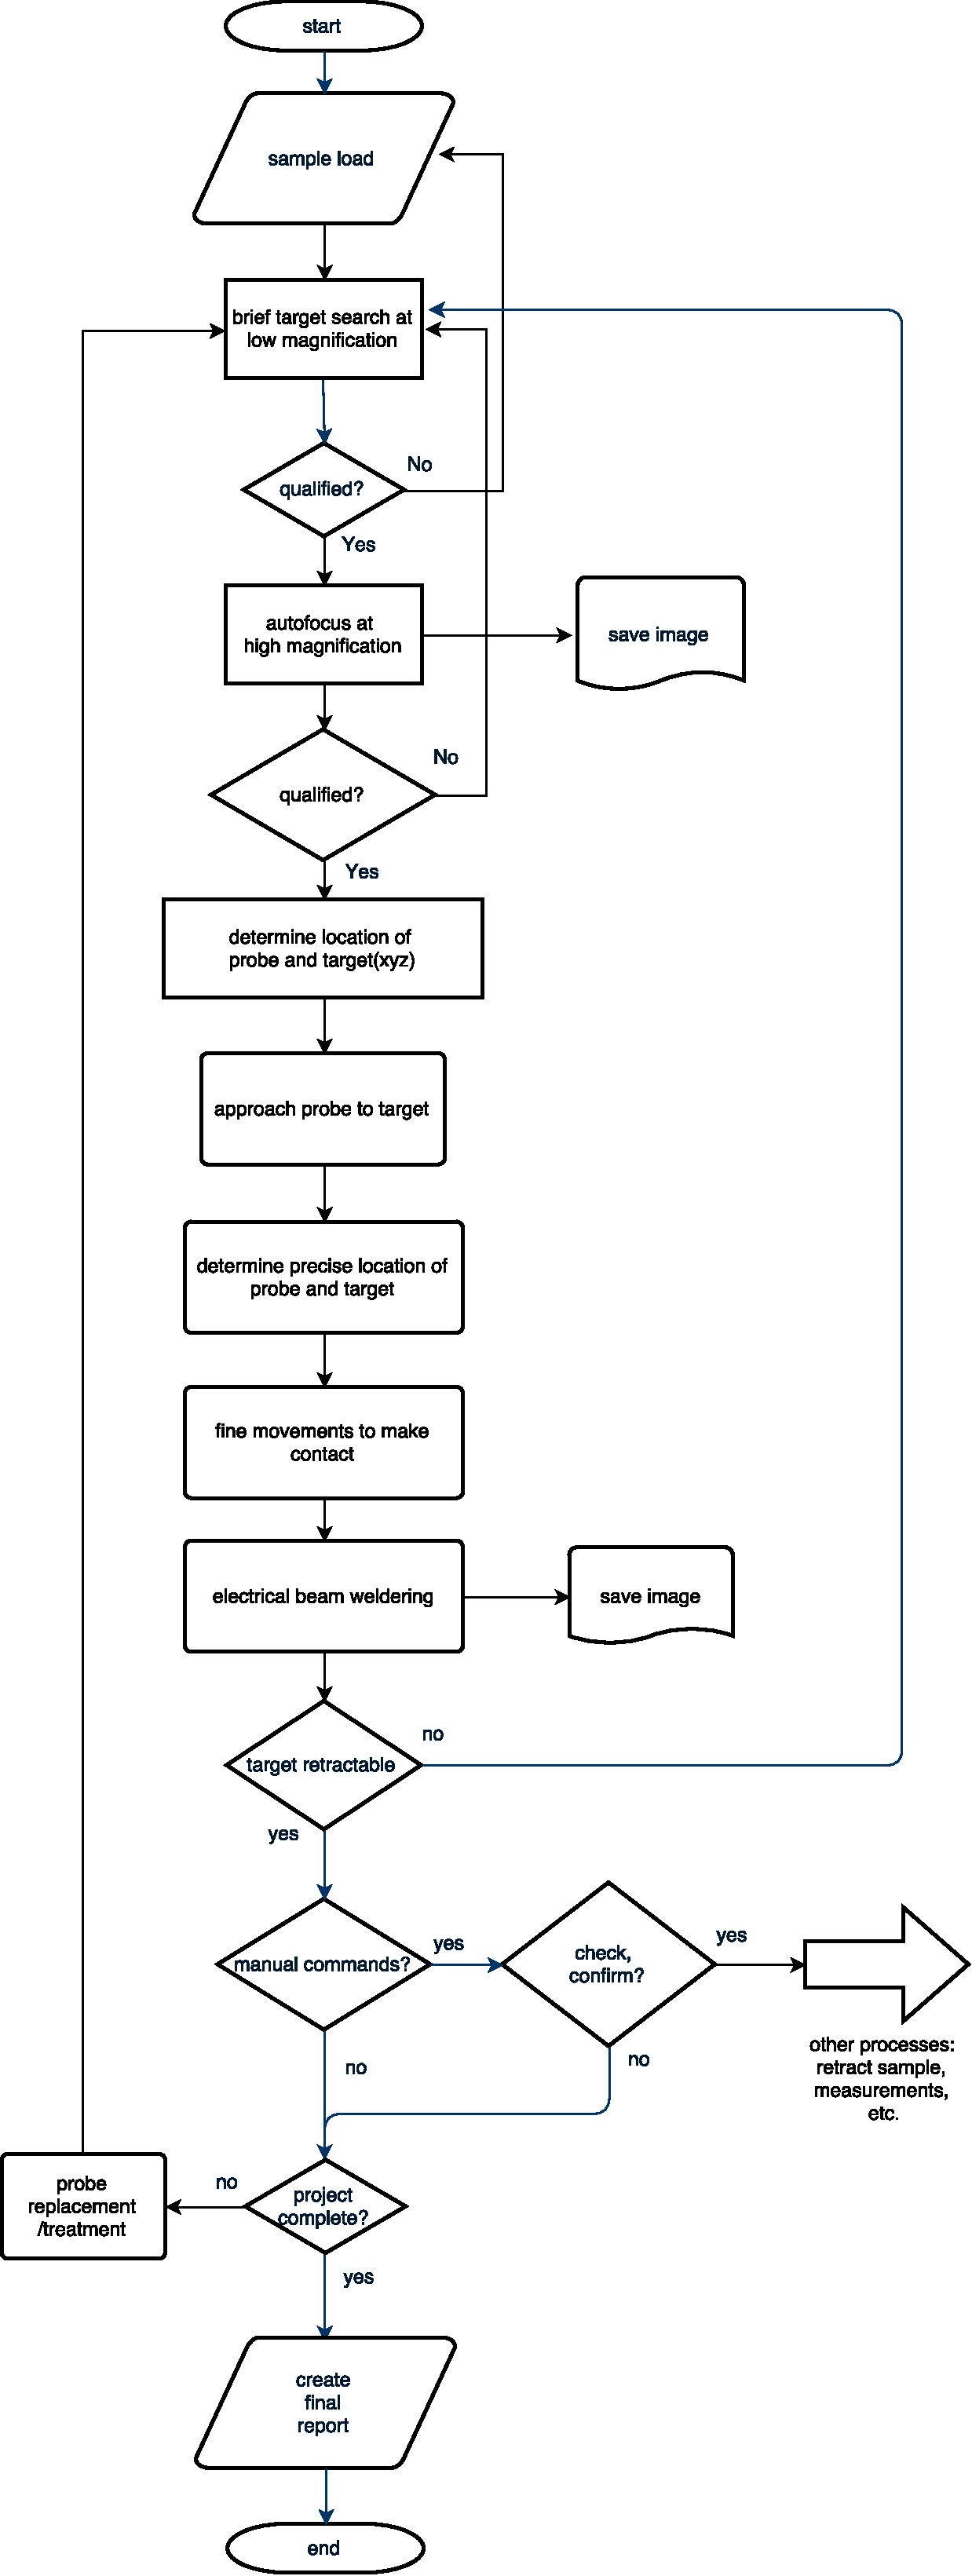
\includegraphics[width=236pt]{figures/figure7_ai}
\caption[AI for Nanomanipulation]
{The workflow for nanoscale manipulations by automation.
\label{fig:7_aiworkflow}}
\end{figure}

During my research toward a PhD degree, I successfully performed thousands of nanoscale operations manually. Most processes are based on the personal experience.  
If we are able to translate our experience into codes for a machine, it is very possible that machines become able to perform the repeatable operations. In Figure \ref{fig:7_aiworkflow}, an example of automation of nanomanipulation is illustrated. In this workflow figure, the machine starts from sample loading, and then performs searching of qualified nanostructure targets, followed by automation of microscopy, second qualification check, autofocus and auto-alignment for high resolution imaging, third qualification check, determining location of probe and target sample, approaching and contacting probe to target, electron beam soldering, retracting a nanostructure target, and many other possible functions. 
Automation of nanoscale handling through SEM and AFM is also under research now. \cite{Fatikow1997Microsystem} We expect that automation will be mature for mass production of future micro- and nano-flexible optoelectronics based on bottom-up technology using various nanomaterials. 

\subsection{Nanomaterials for energy storage in future}
Nanomaterials are superior in offering large surface to volume ratios, decent transport properties, variable physical parameters, and confinement effects resulting from the nanoscale dimensions, and have been extensively studied for energy-related applications, such as solar cells, thermoelectrics, ion batteries, supercapacitors, and gas storage applications.\\
It is expected that the future energy storage is structurally designed down to nanoscale to fully ultilize the nanodimensions: \textit{There is plenty of room at the bottom}. The volumetric capacity could be much higher while at the same time the battery becomes stable and safe. \\
The problems may be solved through:\\
(1) providing a large surface area to boost the electrochemical reaction or molecular adsorption occurring at the solid–liquid or solid–gas interfaces, \\
(2) generating optical effects to improve optical absorption in solar cells, and \\
(3) Ensuring high crystallinity and/or porous structures to facilitate the electron or ion transport and electrolyte diffusion, so as to guarantee that the electrochemical process occurs with high efficiency. It is emphasized that, to further enhance the capability of nanostructured materials for energy conversion and storage, new mechanisms and structures are eagerly awaited. \\
In addition to highlighting the obvious advantages of nanostructured materials, their limitations and challenges for the usage in solar cells, lithium ion batteries, supercapacitors, and hydrogen storage systems are also required to be further investigated in all details.\cite{qifengzhang2013csr}\\


\begin{figure}  
\centering
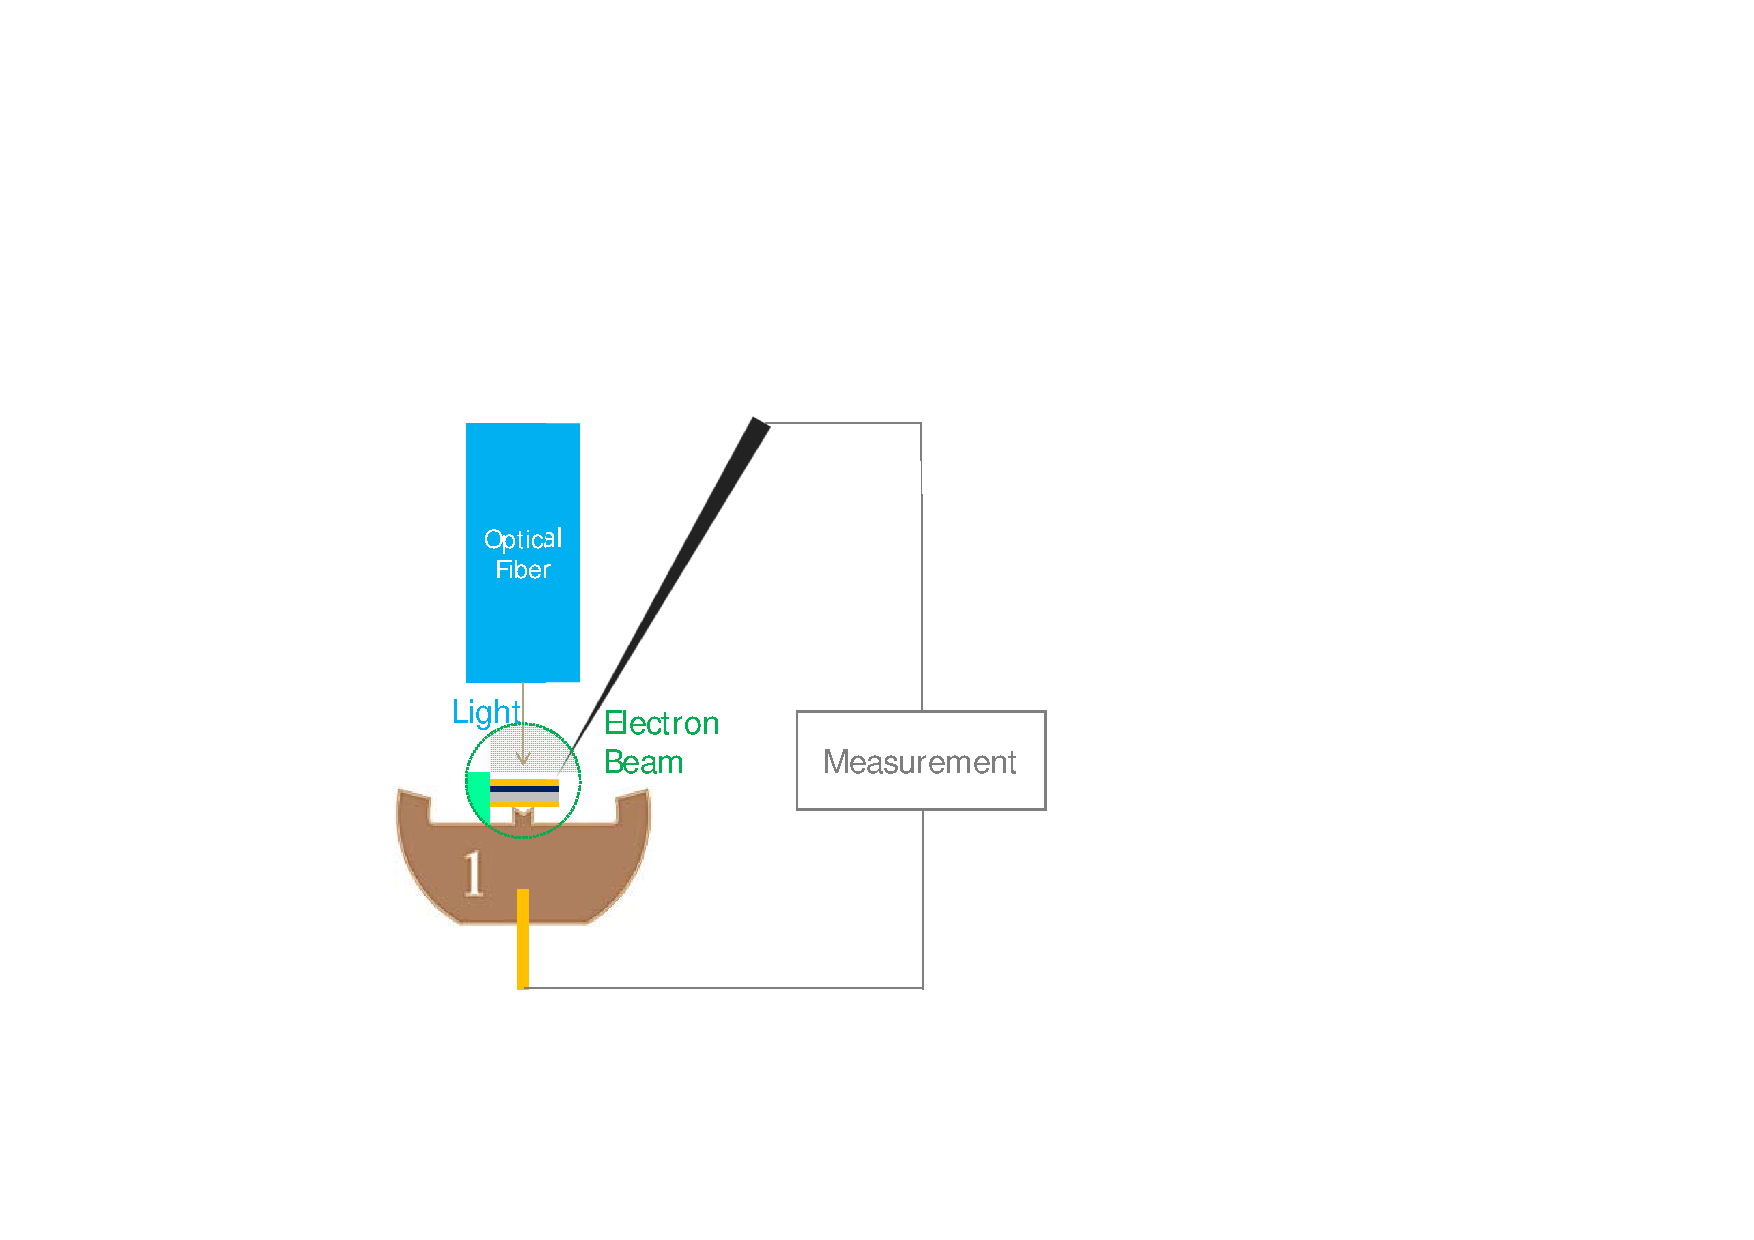
\includegraphics[height=300pt, angle=-90]{figures/figure7_sc}
\caption[Solar cell.]{\textit{in situ} TEM built solar cell. The layered specimen is prepared as a cross section of the solar cell.
\label{fig:7_sc}}
\end{figure}

\subsection{Nanoscale optoelectronics in the future}
All of us are expecting optoelectronics to be integrated into our daily life. To develop an integrated optical interconnect technology and to significantly decrease the energy consumption of future computing systems such paradigm could not be underestimated. The low-loss and high-speed features of optical interconnects would allow for the usage of much greater bandwidths. Taking electrical signals from processors and transferring them into optical/light signals, which are then transmitted via optical waveguides on printed circuit boards, are the urgent steps. This is paving the way for integrating optical and electrical functions, as well as building components directly in the processors. \\
We probably would not get rid of silicon technology because it is still the best choice for microelectronics. However for an optical-electrical transfer, we require many semiconductors with different intrinsic electrical band structures. It is possible to integrate other materials, such as direct and wide band gap materials (such as CdS, ZnO), into silicon electronics. \\
Once the quality of these nanoscale building blocks becomes good enough (especially the present probable inconsistency is eliminated), once the nanoscale manipulation technology finds itself mature enough (mass automated production), the nanoscale optoelectronics should boost into the real market. By simply placing several optoelectronic semiconducting nanoscale building blocks around a processor, optical-electrical signals within a single chip will first be applied to "green" and high-end computing, and then to our daily life necessities. 

%\subsection{Nanomaterials for flexible electronics in future}
%decide not to write this subsection

\subsection{\textit{In situ} probing TEM in the near future}
\color{red}
To make ways for those future applications, experiments and investigations through \textit{in situ} microscopy are fundamental and essential. 

Various materials were tested using \textit{in situ} probing microscopy. Besides Si, CdS, P@GN and ZnO as discussed in previous chapters, many other materials such as \ce{TiO2} nanocrystals, \ce{MoS2} nanosheets, ZnSe/GaP nanowires and CdS/ZnO branched nanostructures also performed clear photocurrent responses, while \ce{SnO2@G} microsheets, Si/C nanospheres, \ce{Cu/Li4Ti5O12} scaffolds, \ce{MoS2/C} nanosheets and N doped graphone showed decent energy storage porfomances.\\

For electrical/optical \textit{in situ} probing TEM experiments, many other samples I measured did not demonstrate strong photocurrent responses. For example, \ce{In2O3}, \ce{ZnS}, boron nitride(BN), \ce{BN-C}, \ce{BCNO}, \ce{CN} with wide/indirect band gap or low conductivity does not respond to our light illumination properly. For BN family materials, strong deep UV laser may excite carriers new results, but for my experiments, some regularly changing current signals were caused by absorbing light energy and heating. \\

Therefore, for the indirect band gap semiconductors, and for the not well-defined band gap materials, the electrical/optical \textit{in situ} probing TEM is expected to detect possible small optoelectronic signals for various optoelectronic applications. It is also expected that the optical fiber plus electrical measuring equipments shall upgrade to collected and processed lower scale signals from smaller (regions of) samples. \\

As I mentioned in Chapter 2, \textit{in situ} photovoltage measurements are also possible to be performed by similar microscopy setup. 


For instance, solar cells are not detailed investigated by \textit{in situ} TEM. One of my experimental design of \textit{in situ} solar cell is presented in Figure \ref{fig:7_sc}. The solar cell can be processed by slicing and FIB to be placed in TEM. \\ 

For physical/chemical \textit{in situ} probing TEM experiments for energy storage, the near future research is more clear but challenging. It is expected that the structure design would be more complicated and space-efficient with higher-level control of structural consistency, and with proper contents of materials. The \textit{in situ} probing experiments for energy storage, including new types of ion-batteries (Aluminum-ion batteries and Magnisium-ion batteries), super-capacitors and pseudocapacitors, are interesting and anticipated. 
\color{black}

